% ============================================================
% Apresentação (defesa TCC) — ~10 min, slides com pouco texto.
% Compilar com pdfLaTeX no Overleaf (tema metropolis já disponível).
% Figura: pareto_front.png (mesma pasta).
% ============================================================
\documentclass[11pt,aspectratio=169]{beamer}

\usetheme{metropolis}
\metroset{block=fill, progressbar=frametitle}

\usepackage[T1]{fontenc}
\usepackage[utf8]{inputenc}
\usepackage[brazil]{babel}
\usepackage{booktabs}
\usepackage{tikz}
\usetikzlibrary{arrows.meta,positioning}

% Realce de coluna/valor na tabela do trade-off
\definecolor{kneecol}{RGB}{234,110,45}

\title{Balanceamento competitivo com preservação de identidade}
\subtitle{Algoritmos Genéticos e NSGA-II em arquétipos de jogos de luta}
\author{Matheus Gimenes de Souza \\ \small Orientador: Prof.\ Dr.\ Everson Scherrer Borges}
\institute{Instituto Federal do Espírito Santo --- Campus Cachoeiro de Itapemirim}
\date{2026}

\begin{document}

\maketitle

% ------------------------------------------------------------
\section{O problema}

\begin{frame}{A tensão central do balanceamento}
  Um jogo competitivo de qualidade precisa de \alert{arquétipos distintos}
  \emph{e} de \alert{equilíbrio}.

  \bigskip
  Mas ao ajustar números para igualar as taxas de vitória, corre-se o risco
  de \textbf{homogeneizar} os personagens.

  \vfill
  \begin{center}
    \Large
    Equilibrar é trivial se todos são iguais.\\
    O desafio é equilibrar \alert{preservando a diferença}.
  \end{center}
\end{frame}

\begin{frame}[standout]
  Um Algoritmo Genético é capaz de atingir equilíbrio competitivo entre
  cinco arquétipos distintos \emph{sem destruir suas identidades funcionais}?
\end{frame}

\begin{frame}{A decisão que evita a circularidade}
  \alert{Medir} a identidade --- nunca \alert{impor}.

  \bigskip
  \begin{itemize}
    \item Desvio ao perfil canônico $\rightarrow$ penalidade \emph{suave} (um objetivo)
    \item Ciclo de vantagens (quem vence quem) $\rightarrow$ medido \emph{post hoc}, fora da otimização
  \end{itemize}

  \vfill
  \footnotesize
  Se a identidade fosse \emph{recompensada}, o AG a ``preservaria'' só por isso ---
  e a resposta seria circular.
\end{frame}

% ------------------------------------------------------------
\section{Método}

\begin{frame}{Cinco arquétipos, um ciclo não transitivo}
  \begin{columns}[c]
  \begin{column}{0.56\textwidth}
  \centering
  \begin{tikzpicture}[
    every node/.style={font=\scriptsize},
    arch/.style={draw=mDarkTeal, fill=mDarkTeal!12, rounded corners,
                 inner sep=3pt, minimum width=1.7cm, align=center},
    win/.style={-{Stealth[length=2mm]}, thick, mDarkTeal},
    win2/.style={-{Stealth[length=1.7mm]}, semithick, kneecol, opacity=0.75}]
    \node[arch] (R)  at (90:2.9)   {Rushdown};
    \node[arch] (CM) at (18:2.9)   {Combo\\Master};
    \node[arch] (Z)  at (-54:2.9)  {Zoner};
    \node[arch] (G)  at (-126:2.9) {Grappler};
    \node[arch] (T)  at (162:2.9)  {Turtle};
    % pentágono externo (vence o vizinho)
    \draw[win] (R)--(CM); \draw[win] (CM)--(Z); \draw[win] (Z)--(G);
    \draw[win] (G)--(T);  \draw[win] (T)--(R);
    % estrela interna (vence o seguinte)
    \draw[win2] (R)--(Z); \draw[win2] (CM)--(G); \draw[win2] (Z)--(T);
    \draw[win2] (G)--(R); \draw[win2] (T)--(CM);
  \end{tikzpicture}
  \end{column}
  \begin{column}{0.44\textwidth}
    \small
    Estrutura pedra-papel-tesoura:\\[2pt]
    \textbf{cada um vence 2 e perde 2}.

    \bigskip
    A seta indica quem vence.

    \medskip
    \footnotesize
    Roster, valores canônicos e ciclo são uma \emph{hipótese} dos autores ---
    verificada \emph{post hoc}, nunca codificada.
  \end{column}
  \end{columns}
\end{frame}

\begin{frame}{Modelo de combate: 1\,vs\,1, tick a tick}
  \centering
  \begin{tikzpicture}[font=\scriptsize]
    \draw[thick] (0,0)--(8,0);
    \foreach \x in {0,2,4,6,8} \draw (\x,-0.08)--(\x,0.08);
    \node[circle,fill=mDarkTeal,inner sep=2.5pt,label=above:{A}] at (1,0){};
    \node[circle,fill=kneecol,inner sep=2.5pt,label=above:{B}] at (6.5,0){};
    \node at (4,-0.5){campo unidimensional (100 unidades)};
  \end{tikzpicture}

  \vfill
  \begin{itemize}
    \item Decisão em duas fases: \alert{intenção} $\rightarrow$ \alert{execução}
          (ATTACK / ADVANCE / RETREAT / DEFEND)
    \item Intenção amostrada pelos \emph{pesos comportamentais} do personagem
    \item Essa amostragem é a \textbf{única} fonte de aleatoriedade
  \end{itemize}
\end{frame}

\begin{frame}{Dois objetivos em conflito}
  \begin{columns}[t]
  \begin{column}{0.5\textwidth}
    \begin{block}{Identidade --- \emph{drift}}
      Distância ao perfil canônico.\\
      \small (menor = mais fiel ao arquétipo)
    \end{block}
  \end{column}
  \begin{column}{0.5\textwidth}
    \begin{block}{Equilíbrio --- \emph{dominance}}
      Nenhum arquétipo domina o roster.\\
      \small (menor = mais equilibrado)
    \end{block}
  \end{column}
  \end{columns}

  \vfill
  \begin{center}
    \Large Balanceamento = problema \alert{bi-objetivo}.
  \end{center}
\end{frame}

\begin{frame}{Duas buscas sobre os mesmos objetivos}
  \begin{columns}[c]
  \begin{column}{0.5\textwidth}
    \centering
    \begin{tikzpicture}[scale=0.8, font=\scriptsize]
      \draw[->] (0,0)--(4.4,0) node[right]{\emph{drift}};
      \draw[->] (0,0)--(0,3.6) node[above]{\emph{dominance}};
      \draw[thick,mDarkTeal] plot[smooth]
        coordinates {(0.25,3.2)(0.7,1.7)(1.5,0.9)(2.6,0.5)(3.8,0.35)};
      \fill[kneecol] (3.9,0.3) circle (2.2pt);
      \node[kneecol] at (3.4,0.9){\footnotesize AG escalar};
      \node[mDarkTeal] at (1.7,2.6){\footnotesize NSGA-II};
    \end{tikzpicture}
  \end{column}
  \begin{column}{0.5\textwidth}
    \small
    \textbf{AG escalar}: soma ponderada\\
    $\rightarrow$ entrega \alert{um} ponto do trade-off.

    \bigskip
    \textbf{NSGA-II}: sem pesos\\
    $\rightarrow$ mapeia \alert{toda} a fronteira de Pareto.
  \end{column}
  \end{columns}
\end{frame}

% ------------------------------------------------------------
\section{Resultados}

\begin{frame}{Baseline canônico: identidade perfeita, equilíbrio ausente}
  \begin{columns}[t]
  \begin{column}{0.5\textwidth}
    \textbf{Identidade} \textcolor{mDarkTeal}{$\checkmark$}
    \begin{itemize}
      \item Validador: \alert{21/21} asserções
      \item \emph{drift} $= 0$
    \end{itemize}
  \end{column}
  \begin{column}{0.5\textwidth}
    \textbf{Equilíbrio} \textcolor{kneecol}{$\times$}
    \begin{itemize}
      \item \alert{0/10} confrontos equilibrados
      \item Rushdown vence 100\% · Turtle vence 0\%
    \end{itemize}
  \end{column}
  \end{columns}

  \vfill
  \begin{center}
    Achado: o ciclo canônico \textbf{não} sobrevive sozinho ao modelo
    determinístico --- apenas \alert{5/10} arestas se sustentam.
  \end{center}
\end{frame}

\begin{frame}{Otimizar só o equilíbrio custa identidade}
  \textbf{AG escalar} (pesos iguais) $\rightarrow$ persegue um único ponto:

  \bigskip
  \begin{itemize}
    \item \alert{10/10} confrontos equilibrados \textcolor{mDarkTeal}{$\checkmark$}
    \item Mas o validador cai para \alert{7/21} e a diferenciação recua (0{,}92)
  \end{itemize}

  \vfill
  \begin{center}
    \Large
    Igualar as vitórias, sozinho, \alert{dissolve} as identidades\\
    --- exatamente a tensão prevista.
  \end{center}
\end{frame}

\begin{frame}{A fronteira de Pareto torna o trade-off explícito}
  \centering
  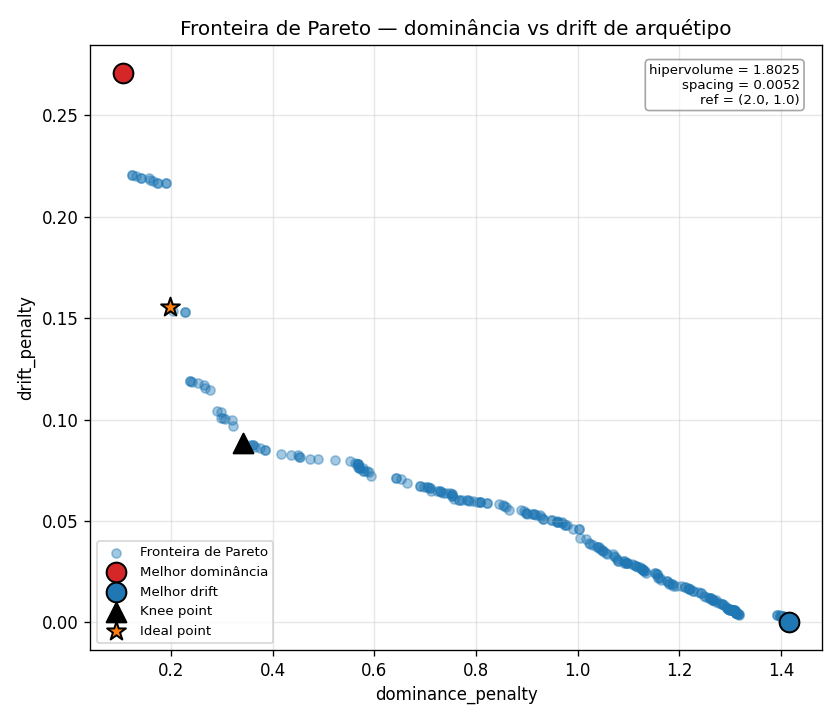
\includegraphics[height=0.72\textheight]{pareto_front.png}

  \footnotesize
  Equilíbrio e identidade \emph{são} objetivos conflitantes --- e o quanto se
  troca de um pelo outro fica \alert{mensurável}.
\end{frame}

\begin{frame}{Lendo o trade-off}
  \centering
  \begin{tabular}{lcccc}
    \toprule
     & Canônico & AG escalar & \textcolor{kneecol}{\textbf{\emph{knee}}} & best\_dom \\
    \midrule
    Desbalanço $\downarrow$   & 1{,}42 & 0{,}01 & \textcolor{kneecol}{\textbf{0{,}34}} & 0{,}11 \\
    Conf.\ eq.\ (/10)         & 0      & 10     & \textcolor{kneecol}{\textbf{2}}      & 9 \\
    Validador (/21)           & 21     & 7      & \textcolor{kneecol}{\textbf{20}}     & 13 \\
    Diferenciação             & 1{,}00 & 0{,}92 & \textcolor{kneecol}{\textbf{0{,}96}} & 0{,}96 \\
    \bottomrule
  \end{tabular}

  \vfill
  \small
  O \alert{\emph{knee point}} reduz o desbalanço de 1{,}42 para 0{,}34
  preservando a identidade quase intacta (\alert{20/21}) ---
  onde o extremo \emph{best\_dom} equilibra mais, mas erode a identidade (13/21).
\end{frame}

\begin{frame}{Robustez: não é sobreajuste ao \emph{fitness}}
  \small Agregado sobre \alert{10 execuções} independentes:
  \begin{itemize}
    \item Cada personagem fica globalmente equilibrado em 90--100\% das execuções
    \item Zerar todos os \emph{hard-counters} de par é o que depende da semente
  \end{itemize}

  \medskip
  \small Validação \alert{fora do laço} (10 sementes novas, ao estilo Ludi):
  \begin{itemize}
    \item \alert{5/5} personagens seguem equilibrados
    \item \alert{9/10} confrontos equilibrados em \emph{todas} as condições
  \end{itemize}
\end{frame}

% ------------------------------------------------------------
\section{Conclusão}

\begin{frame}[standout]
  Sim --- mas sob um trade-off \emph{mensurável}.
\end{frame}

\begin{frame}{Resposta à pergunta}
  \begin{itemize}
    \item Equilíbrio \alert{substancial} é compatível com identidade
          \emph{largamente preservada} (quase intacta no \emph{knee point})
    \item Equilíbrio \alert{total} exige alguma homogeneização
    \item A fronteira permite \textbf{escolher conscientemente} o ponto de operação
  \end{itemize}

  \vfill
  \footnotesize
  \textbf{Limitações}: modelo simplificado (sem \emph{frames}/\emph{mix-ups}),
  5 arquétipos, \emph{round-robin}.\\
  \textbf{Futuro}: coevolução · \emph{quality-diversity} (MAP-Elites) ·
  \emph{restricted play}.
\end{frame}

\begin{frame}[standout]
  Obrigado!

  \vfill
  \small
  Matheus Gimenes de Souza\\
  \texttt{contato.matheusgimenes@gmail.com}
\end{frame}

\end{document}
